\documentclass[conference]{IEEEtran}
\usepackage{cite}
\usepackage{amsmath,amssymb,amsfonts}
\usepackage{graphicx}
\usepackage{booktabs}
\usepackage{array}
\usepackage{textcomp}
\usepackage{url}
\usepackage[hidelinks]{hyperref}
\usepackage{cuted}
\usepackage{capt-of}
\hypersetup{
    pdftitle={QubitChat: A Controlled Evaluation of Grover-Inspired Reranking for Document Retrieval},
    pdfauthor={Anishitha Kovvuri; Bala Rakesh Gundapaneni; Abdul Basith Syed; Jagadeeshbabu Borru; Naga Sravanthi Puppala}
}
\author{
\IEEEauthorblockN{Anishitha Kovvuri,\\
Bala Rakesh Gundapaneni, Abdul Basith Syed,\\
Jagadeeshbabu Borru, Naga Sravanthi Puppala}
\IEEEauthorblockA{Computer Science and Engineering, SRM University AP, 522502, Andhra Pradesh, India\\
Contributing authors: \url{anishitha\_kovvuri@srmap.edu.in};\\
\url{balarakesh\_gundapaneni@srmap.edu.in}; \url{abdulbasith\_syed@srmap.edu.in};\\
\url{jagadeeshbabu\_borru@srmap.edu.in};\\
* Corresponding author(s). E-mail(s): \url{nagasravanthi.p@srmap.edu.in}}
}

\title{QubitChat: A Controlled Evaluation of Grover-Inspired Reranking for Document Retrieval}

\begin{document}
\maketitle

\begin{abstract}
QubitChat is a document-chat prototype combining classical MiniLM embeddings and candidate selection with simulated amplitude amplification. We evaluate retrieval apart from response generation on official SciFact and NFCorpus test sets, with 300 and 323 judged queries. Comparisons cover lexical retrieval, exact cosine, hierarchical navigable small-world indexing, analytical amplification, matched classical sampling, and Grover simulation. The encoder revision, preprocessing, shortlist size, shots, seeds, and statistical protocol were fixed before test evaluation. All reranking methods use the same classical exact-cosine shortlist and fall back to it when no candidates are marked. Reported timing excludes query embedding, corpus encoding, index construction, and response generation; Grover and sampling totals include five seeds, not one online query.\ \IfFileExists{generated/abstract_findings.tex}{On SciFact, the Grover policy changed mean normalized discounted cumulative gain at rank 10 by -0.0003 relative to exact cosine (paired $p$=0.918); the analytical control scored 0.662 and matched classical sampling scored 0.661. On NFCorpus, the Grover policy changed mean normalized discounted cumulative gain at rank 10 by -0.0001 relative to exact cosine (paired $p$=0.600); the analytical control scored 0.295 and matched classical sampling scored 0.295. Across the test sets, SciFact: circuits ran for 101/300 queries; 199/300 used exact-cosine fallback because no candidate met the threshold; NFCorpus: circuits ran for 52/323 queries; 271/323 used exact-cosine fallback because no candidate met the threshold.
}{Numerical findings are generated from the sealed run artifacts.} These results show no retrieval improvement or quantum advantage.
\end{abstract}
\begin{IEEEkeywords}
Amplitude amplification, document retrieval, information retrieval, quantum search, reproducibility.
\end{IEEEkeywords}

\section{Introduction}

Large collections of research papers, technical reports, and other documents require retrieval methods that can identify relevant evidence before a response-generation model is invoked. Retrieval-augmented generation (RAG) systems address this requirement by separating document retrieval from language generation \cite{lewis2020retrieval}. In practice, the retrieval stage includes document extraction, text normalization, chunking, embedding, indexing, scoring, and candidate selection. Each of these stages contributes to the measured cost and must be distinguished from the cost of producing a final natural-language response.

Quantum search is often described using Grover's oracle-query bound, in which amplitude amplification can find marked items with fewer oracle applications under a specified oracle-access model \cite{grover1996search,brassard2002amplitude}. That bound does not by itself replace embedding computation, data loading, oracle construction, circuit compilation, measurement, or ranking. A retrieval experiment that uses classical scores to build a simulated oracle must therefore report those operations separately.

This paper studies that controlled setting. QubitChat is retained as the system platform, while the quantitative retrieval evaluation is deliberately separated from the Gemini response-generation service and from unverified OCR or user-study claims. The primary research questions are:

\begin{enumerate}
    \item Does Grover-inspired reranking improve retrieval effectiveness over exact cosine ranking and a matched classical sampling control when candidate identities and raw scores are fixed?
    \item Can any observed ranking changes be explained by thresholding, marked-state symmetry, finite-shot sampling, score quantization, ties, or candidate construction?
    \item What classical preprocessing, oracle-construction, circuit, transpilation, simulation, and measurement costs are required by the evaluated implementation?
\end{enumerate}

The contributions are threefold. First, we provide an artifact-backed MiniLM evaluation on two public BEIR datasets with published relevance judgments. Second, we specify and test a hybrid reranking policy that keeps classical retrieval distinct from simulated amplification and reports its cosine fallback. Third, we provide matched classical controls and query-derived circuit-resource measurements, including finite-precision effects; padding behavior is analyzed and unit-tested but is not exercised by the power-of-two candidate sizes in the reported runs.

\section{Related Work}

Grover's algorithm provides a foundational example of amplitude amplification for unstructured search \cite{grover1996search}. Brassard et al.~formalized amplitude amplification and its dependence on the fraction of marked states and the number of oracle applications \cite{brassard2002amplitude}. Montanaro surveyed quantum algorithms and their computational assumptions \cite{montanaro2016quantum}, while Biamonte et al.~reviewed quantum machine-learning directions and their data-access requirements \cite{biamonte2017quantum}. These works motivate the mathematical control used here, but they do not establish an end-to-end advantage for the document-retrieval implementation evaluated in this paper.

Neural retrieval and RAG systems use learned text representations to select evidence for downstream generation \cite{reimers2019sentencebert,lewis2020retrieval}. The BEIR benchmark provides heterogeneous information-retrieval datasets and standardized metrics, making it suitable for evaluating whether a retrieval change generalizes beyond a private document collection \cite{thakur2021beir}. BM25 and HNSW are established lexical and approximate-neighbor baselines \cite{robertson2009bm25,malkov2020hnsw}. The present work uses BEIR judgments at parent-document level and reports both conventional retrieval baselines and matched reranking controls.

The distinction between an oracle-query bound and a complete data-processing pipeline is central to this study. Oracle synthesis and reversible data loading can dominate practical resource requirements; consequently, the circuits evaluated here are reported as resource experiments rather than as a claim that sentence embeddings or quantum random access memory have been implemented \cite{seidel2021oracle}.

\section{Datasets and Evaluation Units}\label{sec:dataset}

The quantitative evaluation uses the official BEIR SciFact and NFCorpus archives \cite{thakur2021beir}. SciFact contains scientific claims and evidence documents, while NFCorpus contains nutrition-related questions and documents. Threshold tuning uses held-out judgments only: a deterministic 20\% SHA-256 ordering of SciFact's official train queries using the input prefix \texttt{20260911:scifact:} concatenated with each query ID, and the official NFCorpus dev split. Test membership is defined by positive query IDs in the official \texttt{qrels/test.tsv} files; all 300 SciFact and 323 NFCorpus judged test queries are evaluated, without test-query subsampling.

The shared query JSONL files contain 1,109 SciFact and 3,237 NFCorpus query rows across splits. The positive IDs in the official test qrels select 300 and 323 judged test queries, respectively; all selected IDs have query text. The remaining 809 and 2,914 rows are excluded because they are outside the positive test-qrel ID sets; they are not characterized as unjudged test examples.


Relevance is evaluated at parent-document level. When a document is divided into multiple chunks, the parent score is the maximum cosine score among its chunks; relevance is not assigned to every chunk merely because its parent is relevant. The \texttt{research-v1} run manifests record dataset-file checksums, split/query identifiers, configuration and provenance, source/dependency hashes, and result/circuit hashes; evaluation reads the relevance judgments from the corresponding official, checksummed BEIR qrels files.

\begin{table*}[!t]
\centering
\caption{Dataset and evaluation statistics generated from frozen run manifests.}
\label{tab:dataset}
\resizebox{\textwidth}{!}{\begin{tabular}{lrrrrrrrrrr}
\toprule
Dataset & Corpus & Dev. queries & Test queries & Chunks & Min tokens & Mean tokens & Max tokens & Trunc. & Relevant pairs & Relevant documents\\
\midrule
scifact & 5183 & 161 & 300 & 13503 & 1.0 & 147.3 & 190.0 & 0 & 339 & 283\\
nfcorpus & 3633 & 324 & 323 & 9968 & 1.0 & 148.7 & 190.0 & 0 & 12334 & 3128\\
\bottomrule
\end{tabular}
}
\end{table*}

The application also contains document parsing and OCR paths for text-based and scanned inputs. Those implementation paths are shown in the processing figures, but this paper does not treat the BEIR text benchmark as a quantitative OCR-accuracy evaluation. Similarly, the Gemini generation service is outside the retrieval benchmark and its live-provider latency is not included in the retrieval tables.

\begin{figure*}[!t]
\centering
\begin{minipage}{0.31\textwidth}
    \centering
    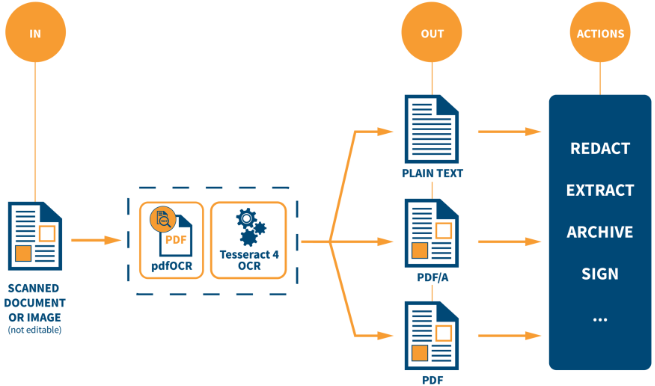
\includegraphics[width=\linewidth]{ocr_text.png}
    \par\small (a) OCR extraction
    \label{fig:ocr}
\end{minipage}
\hfill
\begin{minipage}{0.31\textwidth}
    \centering
    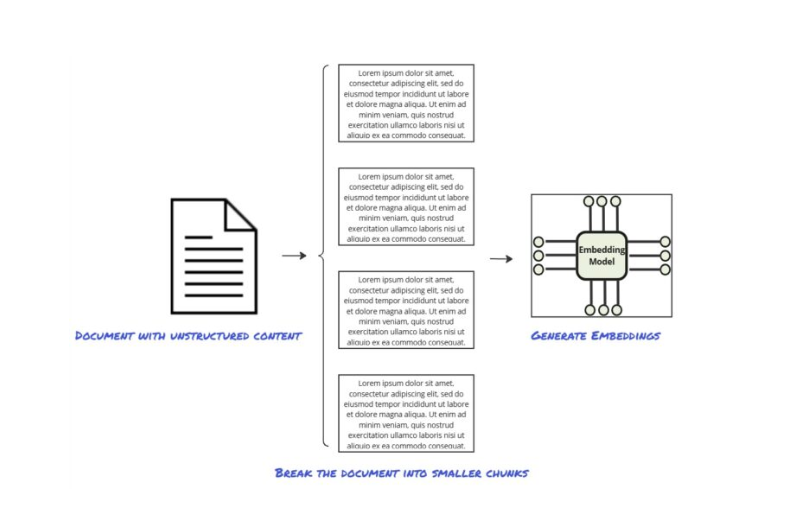
\includegraphics[width=\linewidth]{chunked_doc.png}
    \par\small (b) Chunking
    \label{fig:chunk}
\end{minipage}
\hfill
\begin{minipage}{0.31\textwidth}
    \centering
    
\includegraphics[width=\linewidth]{chat_interaction.png}
    \par\small (c) Interaction
    \label{fig:chat}
\end{minipage}
\caption{Examples of document-processing and conversational-interface stages. These images document the prototype interface and are not quantitative OCR or user-study evidence.}
\label{fig:dataset_samples}
\end{figure*}

\section{Methodology}

\subsection{Preprocessing and MiniLM Embeddings}

The benchmark loader applies Unicode NFKC normalization, whitespace collapse, trimming, and empty-text handling before retrieval. The frozen encoder is MiniLM-L6-v2 \cite{minilm_model}; its pinned model identifier is recorded in Table~\ref{tab:configuration}. The encoder produces 384-dimensional vectors, which are L2-normalized before similarity computation.

Documents are tokenized with the pinned MiniLM tokenizer and segmented into windows of at most 190 content tokens. The implementation reserves two positions for special tokens, reports a nominal 192-token window, and uses a 32-token overlap, corresponding to a stride of 158 tokens. Boundary-safe offset construction and a second tokenization check prevent silent truncation. The measured chunk-length distribution is recorded in the run provenance.

For a query embedding $q$ and chunk embedding $d_i$, cosine similarity is

\begin{equation}
    s_i = \operatorname{cos}(q,d_i) = \frac{q\cdot d_i}{\lVert q\rVert_2\lVert d_i\rVert_2}.
    \label{eq:cosine}
\end{equation}

The highest-scoring chunk determines the score of its parent document. Query vectors for every test query are saved in the run directory, together with query IDs and the model revision, so that the 384-dimensional query representations are explicit audit artifacts rather than implicit intermediate values.

\begin{figure*}[!t]
\centering
\fbox{\parbox{0.94\textwidth}{\centering
\textbf{Text document} $\rightarrow$ \textbf{Unicode normalization and tokenization}
$\rightarrow$ \textbf{190-content-token windows, 32-token overlap}\\[0.35em]
\textbf{Pinned MiniLM encoder} $\rightarrow$ \textbf{L2-normalized 384-dimensional chunk vectors}\\[0.35em]
\textbf{Query--chunk cosine scores} $\rightarrow$ \textbf{maximum score per parent document}
}}
\caption{Text preparation and parent aggregation used in the retrieval evaluation. Application OCR paths are not quantitatively evaluated.}
\label{fig:preprocessing_pipeline}
\end{figure*}

\subsection{Hybrid Retrieval Architecture}

The evaluated pipeline contains five logical stages:

\begin{enumerate}
    \item document loading and deterministic text normalization;
    \item MiniLM tokenization, overlapping chunk construction, and embedding;
    \item classical candidate construction using BM25, exact cosine, or HNSW;
    \item matched reranking using exact cosine, analytical amplification, classical sampling, or Grover circuit simulation;
    \item optional insertion of retrieved text into a response-generation prompt.
\end{enumerate}

The primary Grover, analytical, and sampling comparisons use the same exact-cosine shortlist of 64 parent documents. They are therefore evaluated as matched-candidate rerankers. The classical embedding and shortlist work is not counted as eliminated by the simulated quantum stage.

The measured retrieval path and its fallback are summarized in Fig.~\ref{fig:architecture}.

\begin{figure*}[!t]
\centering
\fbox{%
\begin{minipage}{0.94\textwidth}
\centering
\textbf{Text or PDF input} $\rightarrow$ \textbf{Normalize, extract, and chunk} $\rightarrow$ \textbf{CPU MiniLM embeddings}\\[0.35em]
\textbf{Full-pipeline baselines: BM25, exact cosine, or HNSW}\\[0.25em]
\textbf{Matched reranking: exact-cosine top-64 shortlist} $\rightarrow$
\textbf{classical threshold and marked-index calculation}\\[0.5em]
\begin{minipage}[t]{0.44\linewidth}
\centering
\fbox{\parbox{0.90\linewidth}{\centering
\textbf{No marked candidates}\\
Exact-cosine fallback; no Grover circuit is run.}}
\end{minipage}
\hfill
\begin{minipage}[t]{0.44\linewidth}
\centering
\fbox{\parbox{0.90\linewidth}{\centering
\textbf{At least one marked candidate}\\
Grover simulation, analytical probabilities, or matched classical sampling.}}
\end{minipage}\\[0.5em]
\textbf{Ranking-score transformation and ID tie-break} $\rightarrow$ \textbf{Top-10 documents}
$\rightarrow$ \textbf{optional Gemini generation (outside the benchmark)}\\[0.35em]
\small\textit{Prototype integration (outside the measured retrieval path): React client, FastAPI service, Supabase Auth/Postgres, and Chroma storage.}
\end{minipage}%
}
\caption{Prototype architecture and measured retrieval branch. BEIR corpus text is loaded directly; PDF extraction, OCR, and response generation are application context and are not quantitatively evaluated. Matched reranking methods share a classical exact-cosine shortlist, while the reversible score oracle is measured separately as a resource experiment.}
\label{fig:architecture}
\end{figure*}

\subsection{Marked States and Amplitude Amplification}

For a reranking call with $K\geq2$ valid candidates, the address register has

\begin{equation}
    b = \left\lceil\log_2 K\right\rceil, \qquad B=2^b
    \label{eq:address_space}
\end{equation}

states. If $K$ is not a power of two, addresses $K,\ldots,B-1$ are padding states and are not valid documents. The implementation restricts the cosine threshold to $T\in[0,1]$ and defines the marked set

\begin{equation}
    \mathcal{M}=\{i\in\{0,\ldots,K-1\}:s_i\geq T\}, \qquad M=|\mathcal{M}|.
    \label{eq:marked_set}
\end{equation}

The address qubit with index zero is the least-significant bit in the integer measurement convention used by the implementation \cite{qiskit_bits}. For $0<M<B$, define

\begin{equation}
    \theta=\arcsin\sqrt{\frac{M}{B}}, \qquad
    P_{\mathrm{marked}}(r)=\sin^2((2r+1)\theta).
    \label{eq:amplification}
\end{equation}

The ideal probability of each marked state is $P_{\mathrm{marked}}(r)/M$ and the ideal probability of each unmarked address is $(1-P_{\mathrm{marked}}(r))/(B-M)$. The implementation evaluates the floor and ceiling of the first-peak estimate and chooses the one with the larger marked probability, breaking ties toward the smaller iteration count; it does not use the oversimplified rule $r\approx\sqrt{N}$. The cases $K=0$, $K=1$, $M=0$, and $M=B$ are handled explicitly; no circuit is constructed for an empty or singleton candidate set. The primary retrieval uses $K=64$ and the resource grid uses $K\in\{4,8,16\}$, so all reported candidate counts are powers of two and no padded probability occurs in these experiments. Non-power-of-two padding is covered by unit tests, not by the reported resource grid.

The circuit simulation produces an address distribution. It does not directly produce a sorted relevance list. To obtain a ranking, the implementation combines the signed cosine score with the measured or analytical probability:

\begin{equation}
    r_i=s_i+\beta\max(s_i,0)p_i, \qquad \beta\geq0,
    \label{eq:rank_score}
\end{equation}

where $r_i$ is a ranking score, not a cosine similarity. The marked and unmarked states have group-wise ideal probabilities; amplification alone does not sort all candidates by their individual cosine values. Finite shots, ties, thresholding, quantization, and the signed score transformation can change the final order. The paper therefore reports exact cosine, analytical, and matched classical sampling controls rather than attributing every ranking difference to Grover's algorithm.

\subsection{Oracle Model and Resource Accounting}

In the primary retrieval runs, the threshold predicate is evaluated classically over the 64 cosine scores and the resulting marked indices are supplied to a marked-index phase oracle. The reversible score-lookup oracle described next is a separate resource experiment; it is not used to produce the primary Grover rankings. That resource experiment maps each cosine score $c_i$ and threshold $T$ to $[0,1]$ by $(c_i+1)/2$ and $(T+1)/2$, respectively. For a score width of $w$ bits, it sets $q_i=\operatorname{round}_{\mathrm{even}}((c_i+1)(2^w-1)/2)$ and $q_T=\lceil (T+1)(2^w-1)/2\rceil$. It loads the quantized scores, compares $q_i$ with $q_T$, applies a valid-and-good phase condition, and uncomputes the work registers. It does not implement reversible MiniLM inference, a quantum dot product, or free quantum random access memory. The resource grid enforces an 18-total-qubit cap; the application simulator settings separately default to a 10-address-qubit cap and 64 iterations, and those defaults are not the score-oracle cap. The primary $K=64$ address register requires six qubits, and the saved traces show no resource-limit fallback. The artifacts report address and work qubits, marked-set changes caused by quantization, and separate oracle and search-circuit resources. The reported build/export time covers construction of both circuits, $u/cx$ decomposition for gate counting, QASM serialization, and QASM/QPY file output when enabled; it is an aggregate rather than an isolated oracle-construction time. The retrieval traces separately record phase-oracle construction, transpilation, and simulator execution. A zero-iteration search still reports the separately constructed score oracle; it is not treated as an executed oracle call. These are resource measurements for the implemented oracle model, not physical-QPU performance claims \cite{seidel2021oracle}.

\subsection{Retrieval Algorithm}

The BM25 baseline lowercases text and tokenizes with the ASCII pattern \texttt{[a-z0-9]+}, using $k_1=0.9$ and $b=0.4$ \cite{robertson2009bm25}. HNSW indexes the MiniLM chunk vectors with $M=16$, $efConstruction=100$, and $ef=64$; it retrieves with fourfold chunk overfetch and aggregates duplicate chunks to parent documents by maximum score \cite{malkov2020hnsw}.

\textbf{Algorithm 1: MiniLM Grover-Inspired Document Reranking}

\begin{enumerate}
    \item Normalize the corpus and query using the frozen text policy.
    \item Tokenize documents into 190-content-token windows with 32-token overlap.
    \item Encode document chunks and the query using the pinned MiniLM revision.
    \item Compute cosine scores and aggregate chunk scores to parent documents.
    \item Select the top 64 parent-document candidates using exact cosine similarity.
    \item Compare thresholds 0.5, 0.3, and 0.7 on development nDCG@10 using the matched sampling control; average seeds within query and break ties in that order. The selected threshold is 0.7 on both datasets.
    \item Compute the threshold predicate classically. If no candidate is marked, return the exact-cosine ranking; otherwise construct the address-space circuit for the selected method.
    \item Apply analytical amplification, matched classical multinomial sampling, or Grover simulation.
    \item Apply Eq.~\ref{eq:rank_score}, remove padded addresses, and use document-ID tie-breaking.
    \item Return the top 10 documents and persist candidates, scores, probabilities, seeds, timing, and fallback reasons.
\end{enumerate}

\section{Experimental Protocol}

The frozen configuration is generated directly from the run manifest.

\begin{table*}[!t]
\centering
\caption{Frozen MiniLM retrieval and simulation configuration.}
\label{tab:configuration}
\resizebox{\textwidth}{!}{\begin{tabular}{ll}
\toprule
Setting & Value\\
\midrule
Encoder & sentence-transformers/all-MiniLM-L6-v2@1110a243fdf4706b3f48f1d95db1a4f5529b4d41\\
Embedding dimension & 384\\
Chunk / overlap & 192 / 32 tokens\\
Candidate budget & 64\\
Threshold (SciFact / NFCorpus) & 0.700 / 0.700\\
Development tuning & SciFact: SHA-256 20\% train sample / NFCorpus: official dev\\
Shots & 1024\\
Boost $\beta$ & 2.0\\
Seeds & 0, 1, 2, 3, 4\\
CPU threads & 2\\
Resource-grid total-qubit cap & 18\\
HNSW & efConstruction=100, ef=64, M=16, overfetch=4, seed=0, threads=1\\
Host & Linux; 12 logical CPUs\\
Manifest schema & research-v1\\
\bottomrule
\end{tabular}
}
\end{table*}

The primary metrics are nDCG@10, Recall@10, Recall@64, MRR@10, and P@5. nDCG@10 is the primary endpoint; it uses the published qrel grades directly as gains, while precision and recall treat any positive qrel as relevant, consistent with the BEIR/TREC evaluation convention \cite{thakur2021beir}. Stochastic Grover and classical-sampling repetitions are averaged within each query before statistical inference; seeds and shots are not treated as independent queries. For each dataset, the Holm family contains five paired nDCG@10 comparisons against exact cosine: BM25, HNSW, Grover policy, analytical policy, and sampling policy. The paired-comparison table reports unadjusted two-sided paired sign-randomization $p$-values, unadjusted 95\% percentile confidence intervals from 10,000 paired query-bootstrap resamples, Cohen's $d_z$, and the Holm rejection decision; bootstrap and randomization seeds are 0 and 1, respectively \cite{dror2018harnessing}.

The timing boundary excludes query embedding (test query vectors are precomputed), corpus encoding, one-time HNSW index construction, and Gemini generation. For Grover and sampling, the reported per-query total adds the shared exact-cosine shortlist-selection time to the wall time for all five seeded reranks; it is therefore a five-seed evaluation cost, not single-seed online latency. Other methods are timed once per query. Median and P95 summarize one pass over the test queries and are descriptive, not repeated-run timing estimates. Circuit-resource experiments use five deterministic query-derived score sets per dataset and report unsupported configurations rather than silently changing the qubit or score-bit budget.

\section{Results and Discussion}

\subsection{Retrieval Effectiveness}

The primary retrieval results are generated from all judged test queries and are shown in Table~\ref{tab:retrieval}. The paired comparisons are shown in Table~\ref{tab:matched}; BM25 and HNSW are full-pipeline comparisons, while the three amplification policies use identical exact-cosine candidates and scores. Grover, analytical, and sampling aggregate rows include the defined cosine fallback when no candidate is marked.

\IfFileExists{generated/results_findings.tex}{For SciFact, exact cosine achieved nDCG@10=0.662, while the Grover policy achieved 0.662 (paired difference -0.0003, 95\% CI [-0.0054,0.0051], $p$=0.918). The analytical control was 0.662. Grover circuits ran for 101/300 queries; 199/300 used exact-cosine fallback because no candidate met the threshold. For NFCorpus, exact cosine achieved nDCG@10=0.295, while the Grover policy achieved 0.295 (paired difference -0.0001, 95\% CI [-0.0007,0.0004], $p$=0.600). The analytical control was 0.295. Grover circuits ran for 52/323 queries; 271/323 used exact-cosine fallback because no candidate met the threshold. The analytical and sampling policies use the same no-marked cosine fallback. Aggregate scores therefore evaluate the declared hybrid policies, not circuit execution on every query.
}{}

\begin{table*}[!t]
\centering
\caption{Retrieval effectiveness generated from sealed run artifacts. Reranking-policy rows include cosine fallback when no candidates meet the threshold.}
\label{tab:retrieval}
\resizebox{\textwidth}{!}{\begin{tabular}{llrrrrrr}
\toprule
Dataset & Method & $n$ & nDCG@10 & Recall@10 & Recall@64 & MRR@10 & P@5\\
\midrule
scifact & BM25 & 300 & 0.661 & 0.778 & 0.874 & 0.630 & 0.154\\
scifact & Exact cosine & 300 & 0.662 & 0.817 & 0.924 & 0.617 & 0.163\\
scifact & HNSW & 300 & 0.662 & 0.817 & 0.924 & 0.617 & 0.163\\
scifact & Analytical policy & 300 & 0.662 & 0.817 & 0.924 & 0.617 & 0.163\\
scifact & Classical-sampling policy & 300 & 0.661 & 0.817 & 0.924 & 0.616 & 0.163\\
scifact & Grover policy & 300 & 0.662 & 0.817 & 0.924 & 0.616 & 0.163\\
nfcorpus & BM25 & 323 & 0.305 & 0.146 & 0.217 & 0.507 & 0.277\\
nfcorpus & Exact cosine & 323 & 0.295 & 0.143 & 0.267 & 0.477 & 0.281\\
nfcorpus & HNSW & 323 & 0.291 & 0.140 & 0.263 & 0.473 & 0.280\\
nfcorpus & Analytical policy & 323 & 0.295 & 0.143 & 0.267 & 0.477 & 0.281\\
nfcorpus & Classical-sampling policy & 323 & 0.295 & 0.143 & 0.267 & 0.478 & 0.281\\
nfcorpus & Grover policy & 323 & 0.295 & 0.143 & 0.267 & 0.476 & 0.281\\
\bottomrule
\end{tabular}
}
\end{table*}

\begin{table*}[!t]
\centering
\caption{Paired nDCG@10 comparisons against exact cosine. BM25 and HNSW compare full retrieval pipelines; amplification rows use identical candidates. Differences and confidence limits are in units of $10^{-3}$.}
\label{tab:matched}
\resizebox{\textwidth}{!}{\begin{tabular}{llrrrrrl}
\toprule
Dataset & Comparison & $\Delta$ nDCG ($10^{-3}$) & 95\% CI low & 95\% CI high & raw $p$ & $d_z$ & Holm reject\\
\midrule
scifact & BM25 full pipeline vs. exact & -0.723 & -39.987 & 39.714 & 0.970 & -0.002 & No\\
scifact & HNSW full pipeline vs. exact & 0.146 & 0.000 & 0.438 & 1.000 & 0.058 & No\\
scifact & Analytical vs. exact & 0.000 & 0.000 & 0.000 & 1.000 & 0.000 & No\\
scifact & Sampling vs. exact & -0.851 & -4.294 & 2.825 & 0.621 & -0.027 & No\\
scifact & Grover policy vs. exact & -0.279 & -5.412 & 5.096 & 0.918 & -0.006 & No\\
nfcorpus & BM25 full pipeline vs. exact & 9.834 & -11.046 & 30.968 & 0.360 & 0.050 & No\\
nfcorpus & HNSW full pipeline vs. exact & -3.511 & -10.386 & 0.213 & 0.241 & -0.062 & No\\
nfcorpus & Analytical vs. exact & 0.000 & 0.000 & 0.000 & 1.000 & 0.000 & No\\
nfcorpus & Sampling vs. exact & 0.084 & -0.146 & 0.329 & 0.501 & 0.039 & No\\
nfcorpus & Grover policy vs. exact & -0.149 & -0.706 & 0.356 & 0.600 & -0.030 & No\\
\bottomrule
\end{tabular}
}
\end{table*}

The baseline pattern is dataset-dependent. On SciFact, exact cosine and HNSW have the same nDCG@10 at the reported precision; on NFCorpus, BM25 has higher nDCG@10 than exact cosine (0.305 versus 0.295), while exact cosine has higher Recall@64 (0.267 versus 0.217). Thus, top-rank quality and candidate coverage do not move together in every collection. These point-estimate differences should be interpreted cautiously: every paired confidence interval includes zero, and none of the five comparisons per dataset is rejected by the Holm procedure. For the matched reranking policies, analytical amplification has no nDCG@10 difference at the reported precision, while the Grover and sampling differences are small and statistically unresolved. The result is evidence about reranking a classically selected shortlist, not about quantum candidate discovery.

\subsection{Timing and Circuit Resources}

Table~\ref{tab:timing} reports the timing boundaries stated above. Query embedding, corpus encoding, index construction, and response-generation latency are excluded.

\begin{table}[!t]
\centering
\caption{Retrieval-stage timing generated from per-query traces.}
\label{tab:timing}
\resizebox{\columnwidth}{!}{\begin{tabular}{llrr}
\toprule
Dataset & Method & Median ms & P95 ms\\
\midrule
scifact & BM25 & 39.5 & 78.9\\
scifact & Exact cosine & 19.7 & 27.9\\
scifact & HNSW & 2.3 & 4.5\\
scifact & Analytical & 19.2 & 27.1\\
scifact & Sampling & 19.5 & 27.3\\
scifact & Grover & 21.5 & 450.3\\
nfcorpus & BM25 & 8.5 & 24.5\\
nfcorpus & Exact cosine & 15.4 & 25.1\\
nfcorpus & HNSW & 2.5 & 4.5\\
nfcorpus & Analytical & 15.2 & 25.7\\
nfcorpus & Sampling & 15.4 & 25.9\\
nfcorpus & Grover & 16.0 & 550.8\\
\bottomrule
\end{tabular}
}
\end{table}

HNSW has the lowest reported retrieval median on both datasets, but these measurements exclude index construction and therefore do not establish a lower end-to-end system cost. The Grover P95 values (450.3 ms for SciFact and 550.8 ms for NFCorpus) are substantially above their respective medians; moreover, each Grover timing aggregates five seeded reranks. They should not be read as single-query online latency or as a direct comparison with a physical quantum device.

Table~\ref{tab:resources} reports the query-derived circuit-resource grid. “Q-change” is the number of candidate mark/unmark decisions changed by fixed-point quantization; table entries are medians across five query-derived score sets. “Build/export” includes construction of both circuits, decomposition to the $u/cx$ basis for gate counting, QASM serialization, and enabled QASM/QPY file output. It is an aggregate measurement, not an isolated oracle-construction time. The score oracle uses classically prepared quantized values, so the table is an implementation-resource characterization, not a complete quantum retrieval cost.

The resource grid shows the cost of increasing the encoded problem size. At three score bits, increasing $K$ from 4 to 16 raises the address width from two to four qubits and the median oracle depth from 283 to 5{,}732. At $K=16$, increasing the score precision from three to six bits raises the reported total width from 11 to 17 qubits and oracle depth from 5{,}732 to 8{,}857, with the latter remaining below the configured 18-qubit cap. Search-circuit depth also depends on the query-derived marked set: for the $K=16$, three-bit rows it reaches 11{,}509, unlike the one-layer search circuits in rows with no marked states. These are decomposed simulator-resource counts with classical score loading, not physical-device or end-to-end retrieval costs.

\clearpage
\begin{strip}
\centering
\captionof{table}{Query-derived circuit-resource measurements.}
\label{tab:resources}
\resizebox{\textwidth}{!}{\begin{tabular}{lrrrrrrrrrrrr}
\toprule
Dataset & $K$ & Bits & Qubits & Marked & Q-change & Oracle depth & Oracle 1q & Oracle 2q & Search depth & Search 1q & Search 2q & Build/export ms\\
\midrule
nfcorpus & 4 & 3 & 9 & 1 & 1 & 283 & 244 & 181 & 1 & 2 & 0 & 68.0\\
nfcorpus & 4 & 4 & 11 & 0 & 0 & 360 & 306 & 231 & 1 & 2 & 0 & 114.2\\
nfcorpus & 4 & 6 & 15 & 0 & 0 & 500 & 446 & 337 & 1 & 2 & 0 & 124.7\\
nfcorpus & 8 & 3 & 10 & 1 & 1 & 1278 & 785 & 709 & 1287 & 794 & 715 & 864.5\\
nfcorpus & 8 & 4 & 12 & 0 & 0 & 1609 & 999 & 903 & 1 & 3 & 0 & 500.0\\
nfcorpus & 8 & 6 & 16 & 0 & 0 & 2115 & 1339 & 1201 & 1 & 3 & 0 & 554.0\\
nfcorpus & 16 & 3 & 11 & 1 & 1 & 5732 & 3883 & 3493 & 11509 & 7785 & 7014 & 10973.2\\
nfcorpus & 16 & 4 & 13 & 0 & 0 & 6931 & 4697 & 4239 & 1 & 4 & 0 & 3517.1\\
nfcorpus & 16 & 6 & 17 & 0 & 0 & 8857 & 6015 & 5437 & 1 & 4 & 0 & 4357.5\\
scifact & 4 & 3 & 9 & 2 & 2 & 283 & 244 & 181 & 1 & 2 & 0 & 43.1\\
scifact & 4 & 4 & 11 & 1 & 1 & 323 & 292 & 219 & 1 & 2 & 0 & 50.0\\
scifact & 4 & 6 & 15 & 0 & 0 & 421 & 404 & 301 & 1 & 2 & 0 & 46.2\\
scifact & 8 & 3 & 10 & 2 & 2 & 1278 & 785 & 709 & 1287 & 794 & 715 & 465.3\\
scifact & 8 & 4 & 12 & 1 & 1 & 1557 & 969 & 875 & 1462 & 918 & 825 & 545.5\\
scifact & 8 & 6 & 16 & 0 & 0 & 1855 & 1189 & 1061 & 1 & 3 & 0 & 328.8\\
scifact & 16 & 3 & 11 & 2 & 2 & 5732 & 3883 & 3493 & 11509 & 7785 & 7014 & 6050.4\\
scifact & 16 & 4 & 13 & 1 & 1 & 7285 & 4931 & 4455 & 6128 & 4166 & 3749 & 4206.1\\
scifact & 16 & 6 & 17 & 0 & 0 & 8857 & 6015 & 5437 & 1 & 4 & 0 & 2859.0\\
\bottomrule
\end{tabular}
}
\end{strip}

\subsection{Interpretation and Error Analysis}

The principal diagnostic is whether the Grover and analytical rankings differ from the exact-cosine ranking on identical candidates. When ideal marked-state probabilities are shared within marked and unmarked groups, a ranking change must be explained by the score transformation, threshold boundary, ties, finite shots, quantization, or another explicitly recorded operation. The per-query traces record marked counts, amplification iterations, padded probability, fallback reasons, and per-seed rankings so that these mechanisms can be inspected rather than inferred from aggregate scores.

The experiment also distinguishes approximate HNSW candidate retrieval from exact cosine retrieval, and it records failures and classical fallbacks in the run denominator. A Grover request that cannot be executed within the configured simulator limits is not relabeled as a successful Grover result.

\section{Limitations and Conclusion}

This study is limited to CPU-based classical simulation and public text retrieval judgments. The run manifests record Linux, 12 logical CPUs, and two configured CPU threads, but not the CPU model or RAM; timing results are therefore environment-specific and not fully hardware-reproducible. It does not demonstrate a physical quantum speedup, reversible MiniLM inference, free qRAM, quantitative OCR accuracy, a user study, or live-provider generation quality. The simulated Grover stage receives classical candidate scores and therefore cannot be interpreted as replacing the upstream embedding and candidate-construction work. The BEIR results also do not establish performance on every private document collection or every scanned-document distribution.

On both datasets, the evaluated Grover policy has a slightly lower mean nDCG@10 than exact cosine; its paired confidence interval includes zero, and neither comparison is statistically significant after the declared tests and Holm correction. The evidence therefore establishes no retrieval improvement for this policy and no quantum advantage. The results instead characterize the cost and behavior of a simulated hybrid reranker whose threshold and candidate construction remain classical.

\begin{thebibliography}{99}

\bibitem{lewis2020retrieval}
P. Lewis \textit{et al.}, \textquotedblleft Retrieval-augmented generation for knowledge-intensive NLP tasks,\textquotedblright\ in \textit{Advances in Neural Information Processing Systems}, vol. 33, 2020, pp. 9459--9474.

\bibitem{grover1996search}
L. K. Grover, \textquotedblleft A fast quantum mechanical algorithm for database search,\textquotedblright\ in \textit{Proc. 28th Annu. ACM Symp. Theory Comput.}, 1996, pp. 212--219.

\bibitem{brassard2002amplitude}
G. Brassard, P. H\o yer, M. Mosca, and A. Tapp, \textquotedblleft Quantum amplitude amplification and estimation,\textquotedblright\ in \textit{Quantum Computation and Information}, Contemp. Math., vol. 305. Providence, RI, USA: Amer. Math. Soc., 2002, pp. 53--74, doi: 10.1090/conm/305/05215.

\bibitem{montanaro2016quantum}
A. Montanaro, \textquotedblleft Quantum algorithms: An overview,\textquotedblright\ \textit{npj Quantum Inf.}, vol. 2, Art. no. 15023, 2016, doi: 10.1038/npjqi.2015.23.

\bibitem{biamonte2017quantum}
J. Biamonte \textit{et al.}, \textquotedblleft Quantum machine learning,\textquotedblright\ \textit{Nature}, vol. 549, pp. 195--202, 2017, doi: 10.1038/nature23474.

\bibitem{reimers2019sentencebert}
N. Reimers and I. Gurevych, \textquotedblleft Sentence-BERT: Sentence embeddings using Siamese BERT-networks,\textquotedblright\ in \textit{Proc. EMNLP-IJCNLP}, 2019, pp. 3982--3992.

\bibitem{thakur2021beir}
N. Thakur, N. Reimers, A. R\"uckl\'e, A. Srivastava, and I. Gurevych, \textquotedblleft BEIR: A heterogeneous benchmark for zero-shot evaluation of information retrieval models,\textquotedblright\ in \textit{Proc. 35th Conf. Neural Information Processing Systems, Datasets and Benchmarks Track}, 2021.

\bibitem{robertson2009bm25}
S. Robertson and H. Zaragoza, \textquotedblleft The probabilistic relevance framework: BM25 and beyond,\textquotedblright\ \textit{Foundations and Trends in Information Retrieval}, vol. 3, no. 4, pp. 333--389, 2009, doi: 10.1561/1500000019.

\bibitem{malkov2020hnsw}
Y. A. Malkov and D. A. Yashunin, \textquotedblleft Efficient and robust approximate nearest neighbor search using Hierarchical Navigable Small World graphs,\textquotedblright\ \textit{IEEE Trans. Pattern Anal. Mach. Intell.}, vol. 42, no. 4, pp. 824--836, 2020, doi: 10.1109/TPAMI.2018.2889473.

\bibitem{seidel2021oracle}
R. Seidel \textit{et al.}, \textquotedblleft Automatic generation of Grover quantum oracles for arbitrary data structures,\textquotedblright\ arXiv:2110.07545, 2021.

\bibitem{minilm_model}
Sentence Transformers, \textquotedblleft all-MiniLM-L6-v2 model card,\textquotedblright\ Hugging Face. [Online]. Available: \url{https://huggingface.co/sentence-transformers/all-MiniLM-L6-v2}. Accessed: Sep. 19, 2026.

\bibitem{qiskit_bits}
IBM Quantum, \textquotedblleft Bit ordering in the Qiskit SDK.\textquotedblright\ [Online]. Available: \url{https://quantum.cloud.ibm.com/docs/en/guides/bit-ordering}. Accessed: Sep. 19, 2026.

\bibitem{dror2018harnessing}
R. Dror, G. Baumer, S. Shlomov, and R. Reichart, \textquotedblleft The hitchhiker's guide to testing statistical significance in natural language processing,\textquotedblright\ in \textit{Proc. 56th Annu. Meeting Assoc. Comput. Linguistics}, 2018, pp. 1383--1392, doi: 10.18653/v1/P18-1128.

\end{thebibliography}
\end{document}
